\documentclass[11pt]{article}
\usepackage[margin=0.85in]{geometry}
\usepackage{amsmath,amssymb,graphicx,booktabs,hyperref,microtype}
\usepackage[T1]{fontenc}
\hypersetup{colorlinks=true,urlcolor=blue,linkcolor=blue}
\title{Hardware noise and SIC state-space reconstruction\\\large Circuit simulations, geometry, and diagnostic limitations}
\author{\texttt{cirq\_sic} research record}
\date{18 October 2026}
\begin{document}\maketitle
\begin{abstract}
We compare the probability body inferred from noisy real SIC triple-product
circuits with the true quantum body and random-state SIC tomography.
The procedures estimate different objects once errors are present. With qubit
preparation depolarization at Cirq parameter $p=0.05$, triple reconstruction has
$72.665\%$ of the true volume, while tomography has $81.304\%$. Common coherent
rotations leave triples unchanged despite changing labeled tomography outcomes.
Strong attenuation can make the nominal triple body empty without any failure
of physical quantum dynamics. We provide a tested library pipeline, 39 qubit
scenarios, three four-dimensional checks, compilation and shot-budget comparisons,
and saved counts and scripts. All data are simulated; no hardware was tested.
\end{abstract}

\section{Two different experimental objects}
Let $\Pi_i$ be trace-one SIC projectors in dimension $d$, with $n=d^2$,
$G_{jk}=\operatorname{Tr}(\Pi_j\Pi_k)=(d\delta_{jk}+1)/(d+1)$ and
$T_{ijk}=\operatorname{Re}\operatorname{Tr}(\Pi_i\Pi_j\Pi_k)$.
For ideal SIC outcome probabilities,
\begin{equation}
\rho(p)=(d+1)\sum_i p_i\Pi_i-I,\qquad
(A_i)_{jk}=(d+1)T_{jik}-G_{jk}.
\end{equation}
The quantum body is exactly
\begin{equation}
K_0=\{p\in\Delta_n:A(p)=\sum_i p_iA_i\succeq0\}.
\end{equation}
For Hermitian $X=\sum_jx_j\Pi_j$, the quadratic form is
$\operatorname{Tr}(X\rho X)$. Positivity of $\rho$ implies its nonnegativity;
a negative-eigenvalue eigenvector projector supplies a violating $X$ in the
converse direction. Real triples suffice. Moment bounds alone do not give a
complete mixed-state positivity test in general dimension. Background on SIC
probability geometry and its algebra is given in Refs.~\cite{qbist,algebra}.

Our $\widehat K_T$ substitutes measured, permutation-averaged real triples while
keeping the \emph{ideal} Gram matrix. This is an experimental diagnostic, not a
fit or certificate of a physical SIC. It may be inconsistent or empty.
Tomography instead produces probabilities $q_i(\rho)$ through preparation and
measurement errors. Fixed memoryless circuits give an affine map of the input
density operator, whose nominal ideal-frame inverse can be unphysical.
Its image $K_{\rm tomo}$ need not equal $\widehat K_T$.
All comparisons use the same nominal SIC outcome labels. Recalibrating a frame
changes the coordinate convention and must be reported explicitly.

\section{Circuit design and reproducibility}
Real triples use three independently prepared SIC states, a control Hadamard,
two controlled register swaps, and a final control Hadamard. The measured
expectation is $P(0)-P(1)$. Tomography uses pure-state preparation and a SIC
Naimark measurement unitary. Cirq density-matrix simulation uses complex128
arithmetic~\cite{cirq}. The maintained implementation is \texttt{cirq\_sic.noise}.

Five channel families are swept at $0.01,0.05,0.15$: depolarization, bit flips,
phase flips, phase damping and amplitude damping. Each is applied once after
preparation or after every logical circuit moment. Readout bit flips use
$0.01,0.05,0.15,0.20$. Controls include the ideal case, common $R_z(0.4)$
preparation rotation, and three faults localized to the control or first
system register: 39 qubit cases altogether. Localized register cases are not
silently mapped to tomography, whose register roles differ.

Cirq depolarization shrinks a Bloch vector by $\lambda=1-4p/3$.
Bit/phase flips shrink two axes by $1-2p$; phase damping shrinks transverse
axes by $\sqrt{1-\gamma}$. Amplitude damping has
$M=\operatorname{diag}(\sqrt{1-\gamma},\sqrt{1-\gamma},1-\gamma)$,
$t=(0,0,\gamma)$. Equal channel parameters are not equal infidelities or
physical durations. Rotations are specified in radians.

Preparation noise acts only on system qubits, after preparation. An independent
Kraus test caught that Cirq can pack the control Hadamard into the preparation
moment; we explicitly split this moment to insert anisotropic noise correctly.
Moment noise includes idle qubits and final basis rotations. The main sweep uses
logical dense gates and CSWAPs; rates are per moment of that schedule, not native
error rates. A supplementary CZ-gateset compilation has unrestricted connectivity
and no device routing or duration calibration.

For $d=2$ all 64 ordered settings are retained before symmetrization, at 4096
shots per setting. Tomography uses 384 Haar pure states and 4096 shots per state.
Exact channel expectations and sampled counts are both stored. Binomial and
multinomial draws from exact circuit probabilities reproduce terminal measurement
statistics for these fixed, memoryless circuits. They do not model drift or
correlated shots. The seed is 20261018. The recorded environment is Python 3.14.2,
NumPy 2.3.5, SciPy 1.16.3 and Cirq 1.6.1.

The default tomography budget is six times the triple budget; no efficiency
advantage is claimed from this comparison. Supplementary data use 682 tomography
shots per state, or 261888 total, versus 262144 triple shots. Equal shots still
do not imply equal gate, qubit, timing or calibration cost.
For selected cases we generate 100 parametric binomial bootstrap tensors.
Each independent setting is resampled once before permutation averaging.
Endpoint empirical probabilities remain endpoints; percentile ranges are
conditional sampling summaries, not calibrated coverage guarantees.

\section{Metrics and explicit failure handling}
\paragraph{Tensor consistency.}
Metrics include RMSE and maximum error against truth, raw permutation RMS,
$T_{iii}=1$ residuals, $T_{iij}=G_{ij}$ residuals, and closure violations
$\sum_iT_{ijk}-dG_{jk}$. They test ideal SIC identities, not just precision.
Symmetry-compressed data cannot reveal unmeasured order violations.

\paragraph{Full-dimensional geometry.}
From $p_*=\mathbf1/d^2$ we sample uniform directions in the sum-zero hyperplane,
using 4096 common directions for qubits. Radius is limited by either the PSD
boundary or the simplex. Whitening the center pencil reduces the PSD boundary
to a minimum-eigenvalue calculation. Distances are Euclidean in probability
coordinates. We report radial RMSE, sampled maximum radial discrepancy, radius
ratio extrema, relative volume and Jaccard overlap. The maximum radial
 discrepancy is not Hausdorff distance. With $m=d^2-1$,
\begin{equation}
\frac{V_T}{V_0}=\frac{\mathbb E r_T^m}{\mathbb E r_0^m},\qquad
J=\frac{\mathbb E\min(r_T,r_0)^m}{\mathbb E\max(r_T,r_0)^m}.
\end{equation}
A paired delta-method Monte Carlo standard error accompanies volume ratios;
it excludes shot uncertainty. High-dimensional powers of radii can make
Monte Carlo convergence slow, requiring more directions and repeated seeds.

If either center is not strictly feasible, radial metrics are withheld.
This does not in general prove emptiness. A sufficient separate certificate is
$\max_i\operatorname{Tr}A_i<0$: every simplex combination then has negative
trace. This certificate is incomplete. No general SDP feasibility search or
adaptive recentering is implemented.

\paragraph{Tomography.}
We report paired total variation, empirical centroid shift, sorted covariance
axis ratios, triple-pencil acceptance fraction and nominal ideal-inversion
physicality. No positivity projection conceals unphysical inversions.
A full-rank affine fit to known ideal input probabilities supplies singular
values, center translation and residual; for qubits its determinant estimates
the affine-ball volume. A small residual neither proves complete positivity
nor distinguishes preparation and measurement errors. Covariance ratios also
depend on input coverage, unlike singular values of a correctly specified fit.

Qubit hull volume is compared with the true ball and the ideal hull of the same
states. Our ideal 384-state hull covers $96.896\%$ of the true volume, illustrating
finite-coverage bias. Shot noise can inflate hulls or create unphysical inversions.
Beyond qubits, pure states are not the whole mixed-state boundary; a pure-state
cloud is not a uniformly sampled full boundary.

\section{Analytic mechanisms and counterexamples}
\subsection{Preparation depolarization}
For tetrahedral Bloch vectors $n_i$, write
$\rho_i=(I+\lambda n_i\cdot\sigma)/2$. Then
\begin{equation}
T'_{ijk}=\lambda^2T_{ijk}+(1-\lambda^2)/4.
\end{equation}
In coefficient coordinates separating the uniform direction and its orthogonal
complement, the nominal real pencil has a scalar block 1, a traceless block
$(\lambda^2-2/3)I_3$, and off-diagonal coupling scaled by $\lambda^2$.
Its inferred Bloch radius relative to truth is
\begin{equation}
R_T=\frac{\sqrt{3\lambda^2-2}}{\lambda^2},\qquad
R_{\rm tomo}=\lambda\quad (\lambda>0,\ \lambda^2>2/3).
\end{equation}
At $p=0.05$, volumes are $0.726648$ and $0.813037$; at $p=0.10$, they are
$0.300903$ and $0.650963$. For $\lambda^2<2/3$, the constant traceless principal
block is negative, so the nominal triple body is empty. At equality it collapses
to the center. The small-positive-$p$ threshold is
$p=\tfrac34(1-\sqrt{2/3})\simeq0.13763$.
The channel and its tomography image remain physical. The inconsistency arises
from applying ideal-SIC identities to mixed, non-SIC preparations.

\subsection{Readout attenuation}
A control bit flip with probability $e$ gives $T'=sT$, $s=1-2e$. In any dimension,
\begin{equation}
A_s(p)=sA(p)+(s-1)G,\qquad \alpha=\frac{(d+1)s-d}{s}.
\end{equation}
For $d/(d+1)<s\le1$, the inferred body is a contraction by $\alpha$ about $p_*$,
with volume ratio $\alpha^{d^2-1}$. For $s<d/(d+1)$ every pencil has negative
trace, certifying emptiness. The qubit threshold is $e=1/6$.
At $e=0.05$ the triple volume is $0.470508$.
Independent readout flips on the two SIC output bits instead give nonuniform
confusion eigenvalues $s,s,s^2$, so tomography has volume $s^4=0.6561$.
These are different circuit/readout responses, not different quantum kinematics.
Independently calibrated attenuation could be divided out, amplifying variance
by $1/s^2$. Repeated-index triples alone cannot safely calibrate it if preparation
purity and cycle-test gates are also faulty.

\subsection{Gauge blindness and non-identifiability}
A common unitary conjugation leaves all triple products invariant. In the
$R_z(0.4)$ experiment the tensor and body agree with truth to roundoff while
paired tomography has mean TV error $0.08006$. The full tomography body also
remains the same ball: shape alone misses this rotation too. Known input labels
or an external reference frame are necessary.
For qubit Bloch vectors,
\begin{equation}
\operatorname{Re}\operatorname{Tr}(\rho_i\rho_j\rho_k)
=\tfrac14(1+r_i\cdot r_j+r_j\cdot r_k+r_k\cdot r_i).
\end{equation}
A preparation channel $r\mapsto Mr+t$ therefore enters through $M^TM$, $M^Tt$
and $t^Tt$. Real triples cannot determine a common output orthogonal orientation;
complex conjugation preserves their real parts as well. Ancilla contrast loss
and readout attenuation may be confounded. Volume or anisotropy alone does not
uniquely identify a noise mechanism.

\section{Numerical findings}
Table~\ref{tab:summary} gives exact-channel qubit results at parameter 0.05,
plus ideal and coherent controls. Dashes mean an invalid center, not zero volume.
$V_{\rm tomo}$ is the fitted affine-ball volume. Moment noise can violate
permutation symmetry despite an identical channel on each qubit, because
controlled swaps expose registers differently.
\begin{table}[htbp]\centering\small
\begin{tabular}{llrrrr}
\toprule
Channel & Placement & $V_T/V_0$ & $V_{\rm tomo}/V_0$ & TV & $\epsilon_{\rm perm}$ \\
\midrule
ideal & none & 1.000 & 1.000 & 0.000 & 0.0000 \\
depolarizing & preparation & 0.727 & 0.813 & 0.017 & 0.0000 \\
depolarizing & moment all & -- & 0.562 & 0.044 & 0.0100 \\
bit flip & preparation & 0.652 & 0.810 & 0.021 & 0.0000 \\
bit flip & moment all & -- & 0.461 & 0.059 & 0.0133 \\
phase flip & preparation & 0.657 & 0.810 & 0.020 & 0.0000 \\
phase flip & moment all & -- & 0.810 & 0.020 & 0.0108 \\
phase damping & preparation & 0.942 & 0.950 & 0.005 & 0.0000 \\
phase damping & moment all & 0.498 & 0.950 & 0.005 & 0.0042 \\
amplitude damping & preparation & 0.855 & 0.903 & 0.014 & 0.0000 \\
amplitude damping & moment all & 0.551 & 0.735 & 0.046 & 0.0073 \\
bit flip & readout & 0.471 & 0.656 & 0.034 & 0.0000 \\
coherent z & preparation & 1.000 & 1.000 & 0.080 & 0.0000 \\
\bottomrule
\end{tabular}

\caption{Selected qubit simulations. TV uses paired ideal/noisy probabilities;
$\epsilon_{\rm perm}$ is raw permutation RMS.}\label{tab:summary}
\end{table}
\begin{figure}[htbp]\centering
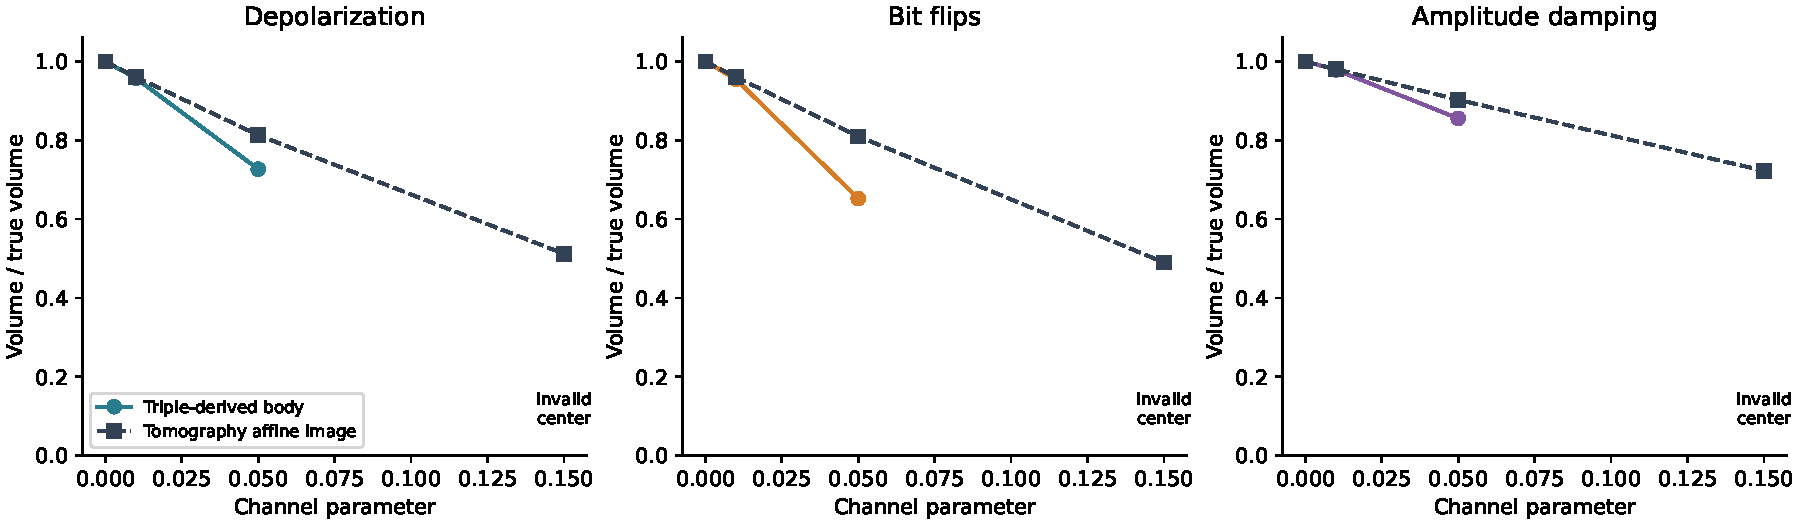
\includegraphics[width=\linewidth]{volumes.pdf}
\caption{Preparation noise: triple and tomography volumes. Lines connect tested
parameters. The invalid depolarizing center at 0.15 is analytically an empty body.}
\end{figure}
\begin{figure}[htbp]\centering
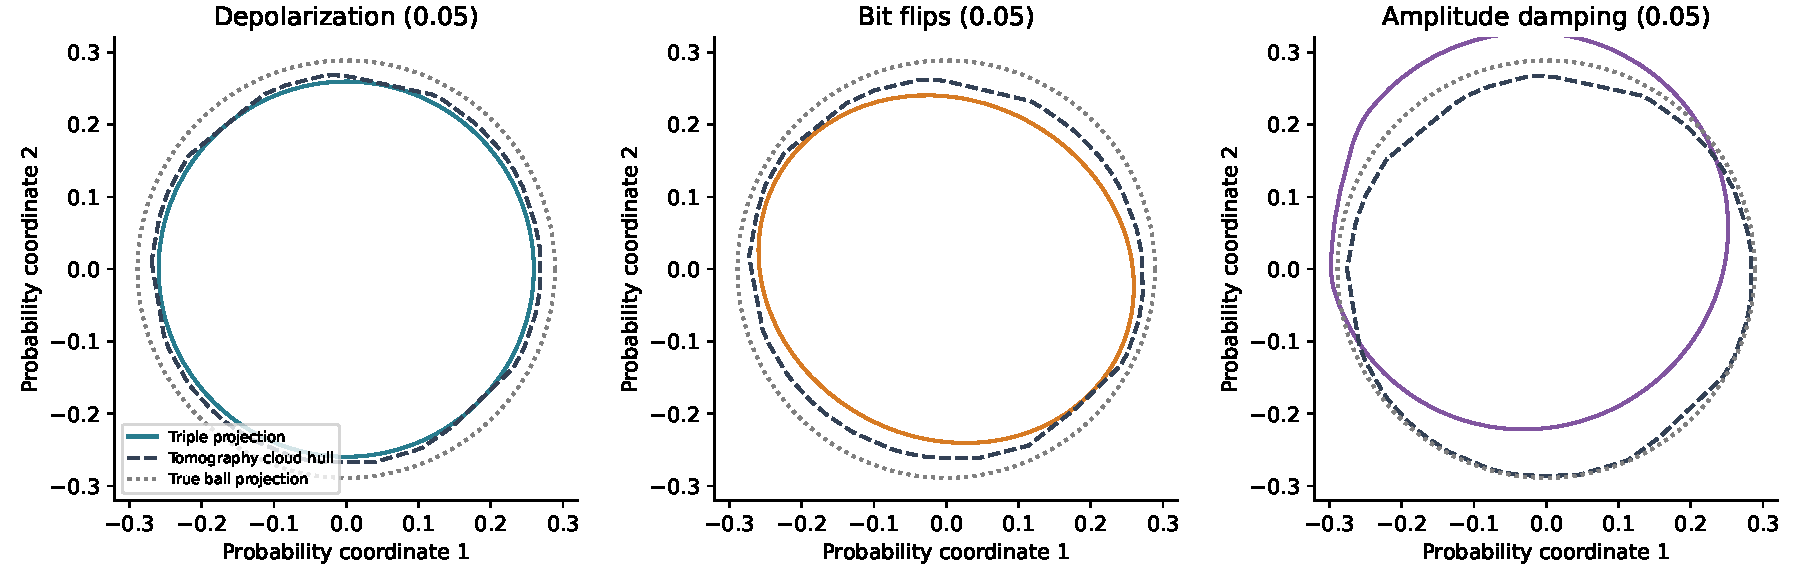
\includegraphics[width=\linewidth]{projections.pdf}
\caption{Two-coordinate projections, not sections, at parameter 0.05. Triple
boundaries use 12000 radial endpoints; tomography uses a 384-state hull. Dotted
circles show truth. Finite boundary/cloud sampling creates inward bias.}
\end{figure}

Amplitude damping recovers the expected tomography singular values and
translation, with volume $(1-\gamma)^2$. At $\gamma=0.05$ its triple volume is
about $0.8554$, versus $0.9025$ for tomography. Bit and phase flips have equal
physical determinant volume but differently oriented contraction. Their finite
Monte Carlo triple-volume estimates should be assessed with sampling errors,
not interpreted as a robust difference in total volume.

At readout error 0.15, exact triple volume is $0.002915$; 13 of 100 bootstrap
centers are invalid. At 0.20 all 100 are invalid. Ideal-case bootstrap volume
percentiles are $[0.9643,1.0168,1.0588]$. These illustrate sensitivity of nonlinear
geometry estimates, particularly near feasibility boundaries; they are not an
interval-coverage validation.

For $d=4$, each exact-channel check uses 816 unordered settings. Ideal recovery
has maximum tensor error about $2\times10^{-15}$. A 1\% control readout error
gives volume ratio $0.27877$, explained by $(0.9/0.98)^{15}$.
Local preparation depolarization at 1\% gives $0.14034$ with directional Monte
Carlo standard error $0.00542$ on 2048 rays. This is exploratory, not a precision
estimate. No $d=4$ tomography cloud or ordered-asymmetry sweep is claimed.

Compilation to the CZ target gateset increases the qubit triple circuit from
4 to a mean 43 moments. With depolarization after each compiled moment, parameter
0.001 gives volume $0.36942$; at 0.01 the body is certified empty by negative
trace. These 20-setting symmetry-compressed checks demonstrate schedule
sensitivity, not predictions for a specific chip. Native routing and durations
remain to be modeled.

\section{Practical hardware protocol}
The method is useful as a structured consistency test and comparative benchmark:
\begin{enumerate}
\item Fix physical qubits, native compilation, routing, timing and nominal SIC
labels. Record circuit depth and gate counts; interleave settings and repeats
to separate drift from index dependence.
\item Acquire independent control contrast/readout and preparation purity or
pair-overlap checks. Include repeated-index triples and deliberate register
permutations before assuming tensor symmetry.
\item Compare raw identity and permutation residuals with shot uncertainty.
Inspect feasibility before plotting. Publish failures and certificates beside
geometry; do not smooth an inconsistent tensor into a plausible body.
\item Sweep depth, idle delay, register assignment and compiler settings.
Use anisotropy, translation, attenuation and order violations as features;
assign mechanisms only after interventions distinguish competing explanations.
\item Acquire labeled-state tomography under a recorded resource budget.
Compare paired error, affine fits, nominal physicality and coverage, not only
shape. Use held-out states or repeats to validate hardware model predictions.
\item For physical frame reconstruction, calibrate the Gram matrix and dual
frame, or jointly fit a constrained gate/SPAM model. Report raw versus fitted
geometry and model uncertainty. Such fitting is not implemented here.
\end{enumerate}

\section{Limitations and continuation}
The current tools assume fixed memoryless channels and independent shots. They
omit drift and leakage, and require custom models for crosstalk or correlated
errors. Circuit helpers accept power-of-two dimensions and pure inputs, avoiding
silent postselection of padded outcomes. Dense tensors cost $O(d^6)$ storage;
ordered settings cost $d^6$, and density matrices scale exponentially in qubits.
The default 4096-setting guard blocks accidental large studies.

Uniform-center failure needs SDP feasibility or recentering for general tensors.
High-dimensional volume estimates need convergence studies. Near-singular PSD
boundaries make bootstrap inference nonregular; repeated simulation experiments
are needed to assess coverage. Beyond qubits, mixed-state ensembles or validated
channel models are needed to infer the full body from tomography clouds.
Priority next work is timing-aware native-device compilation, calibrated
interventions, and ordered $d=4$ data. Arbitrary Cirq noise models and compilation
callbacks are already supported, so these can use the same analysis pipeline.

\appendix
\section{Reproduction and validation}
The study folder is \texttt{research/noise\_state\_space/}. Run
\texttt{run\_study.py}, \texttt{analyze\_results.py}, and \texttt{supplementary.py}
from the repository root; compile this document from its \texttt{report/}
directory. NPZ files preserve states, settings, exact probabilities and counts;
JSON files preserve metrics, failures, versions and seeds. The original prototype
is archived as \texttt{pipeline.py}; maintained code is \texttt{cirq\_sic/noise.py}.
The public API and limitations are in \texttt{docs/noise\_state\_space.md}.

All 283 repository tests pass. New tests validate independent Kraus predictions
for six channel/unitary families, analytic volumes, amplitude-damping affine
parameters, coherent blindness, raw asymmetry, readout maps, shot/bootstrap
reproducibility, compilation, invalid centers, singular clouds and resource guards.
The regression run exposed a pre-existing persistence issue: repeated probability
normalization changed values by an ulp on JSON reload. Already-normalized values
are now preserved at machine precision, with a dedicated regression test.
No hardware validation or confidence-interval coverage claim follows from these tests.

\begin{thebibliography}{9}
\bibitem{qbist} D. M. Appleby, \AA. Ericsson and C. A. Fuchs,
\emph{Properties of QBist State Spaces},
\href{https://arxiv.org/abs/0910.2750}{arXiv:0910.2750}.
\bibitem{algebra} D. M. Appleby, S. T. Flammia and C. A. Fuchs,
\emph{The Lie Algebraic Significance of Symmetric Informationally Complete Measurements},
\href{https://arxiv.org/abs/1001.0004}{arXiv:1001.0004}.
\bibitem{cirq} Google Quantum AI, \emph{Noisy Simulation in Cirq},
\url{https://quantumai.google/cirq/simulate/noisy_simulation}, accessed 18 October 2026.
\end{thebibliography}
\end{document}
